\chapter{\label{cnn} Machine learning for continuous wave searches}
%%%%%%%%%%
%%%%%%%%%%

%--------------------------
% Introduce machine learning
%----------------------------

Machine learning is a term which was used by Arthur Samuel in 1959. 
He described it as a "Field of study that gives computers the ability to learn without being explicitly programmed" \citep{}.
This can be though of as a subset of artificial intelligence. 

With the development in computing in recent years, including GPUs and the languages used to program with them, machine learning has become more accessible. 

%%%%%%%%%%%
%%%%%%%%%%%
\section{\label{machine:nn}Neural networks}
%%%%%%%%%%%
%%%%%%%%%%%


Throughout this section I will summarise one machine learning technique which are known as Neural networks. 
Neural networks, as the name may suggest, was developed as a way for a computer to mimic the neurons in the brain.
To understand why this would be useful, I will give short example which will be followed through this section.
A good example used extensively in explanations of neural networks is the ability to identify hand written digits.
This is a simple task which a brain can complete with ease. 
However, writing a traditional algorithm to perform this same task is very difficult. 
The algorithm would have to identify a particular shape, which has a huge amount of variation.
For example, any number could be written at a slightly different angle or the number 9 could have a much longer tail etc.
This is where a neural network can help. 
These can be trained in a similar way to a human brain. 
This is where in a lifetime many examples of different symbols are seen and each time a new one is seen the brain `updates' itself based on what is observed. 
This process is essentially replicated for a neural network, where the algorithm can be updated such that it can correctly identify each digit.

To explain how a neural network can be updated, we need to start with the operation of a single neuron.


\begin{itemize}
    \item introduce machine learning as a technique with previous examples
    \item general idea, train a NN on lots of data
    \item GPU development allowed these to train fast and be useful
    \item General intended application to CW searches
    \item redue affect of instrumental artefacts
\end{itemize}

%%%%%%%%%
%%%%%%%%%
\subsection{\label{machine:nn:neuron}Neurons}
%%%%%%%%%
%%%%%%%%%

Neurons are the building blocks of any neural network.
They perform simple operations on any number of input values and then output a single value.
The output $o$ of a neuron is defined by the equation,

\begin{equation}
    o = f\left(b + \sum_{i=1}^{N} w_i x_i  \right),
    \label{machine:nn:neuron:equation}
\end{equation}

where $b$ is the bias, $x$ is the input, $w$ is the weights, $f$ is the activation function and $o$ is the output.
Here the input $x$ represents either the data which is input, i.e the pixels of the image which contains the digit in the example above, or the output of another neuron.
The weights $w$ then represents how important each of those data points are to this problem, or specifically this neuron. 
The bias $b$ is then just an extra factor which can shift the data by a fixed value.
The activation function $f$ is then a function which can have many forms, in the simplest case in a neuron known as a `perceptron', it provides a cut where any value above a given threshold is 1 and any below is 0. 
However, there are many different types of activation functions which can be applied to different situations.
This will be explained in more detail in Sec.~\ref{machine:nn:activation}.

\begin{figure}[h]
    \centering
    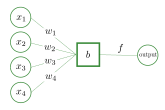
\includegraphics[width=0.6\columnwidth]{C4_cnn/neuron.pdf}
    \caption{Basic neuron}
    \label{machine:nn:neuron:plot}
\end{figure}

In the example in Fig.~\ref{machine:nn:neuron:plot} I have shows a neuron which has 4 input variables, or 4 input data points. 
When a network is trained, or when it learns, the weights applied to each of the inputs and the bias are updated to better represent the input data.
This training procedure is explained in more detail in Sec.~\ref{machine:nn:training}
Many neurons are then used in combination with each other to develop a neural network which can be applied to more complex problems.

%%%%%%%%%%%%%%%%%%%%
\subsection{\label{machine:nn:structure}Network structure}
%%%%%%%%%%%%%%%%%%%%

The structure of the network is defined by the user and there is not set way to design the network.
However, in general the complexity of the network reflect the complexity and size of the input data.
If there is a small number of training examples and a large and complex network, it may be able to learn the input data set as opposed the the general information that they represent.

Neural networks are structured in features called layers, sometimes known as fully connected layers. 
These are rows of $N$ neurons which all take the same input such that there is $N$ output values.
An example of a simple neural network is shown in Fig.~\ref{machine:nn:structure:plot}.
The first layer is the input layer, this is just the input data.
In the example of hand drawn digits, this would be the pixels from the image of the digit.
The final layer represents the information that you intend the network to extract from the input data. 
In the hand drawn digit example, this could have 10 output values corresponding to each digit 0-9. 
Each of these outputs is then a value which is related to the probability of that digit being present in the image.  

\begin{figure}[h]
    \centering
    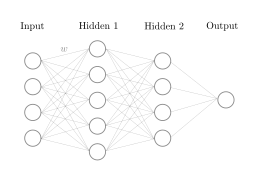
\includegraphics[width=\columnwidth]{C4_cnn/simple_network.pdf}
    \caption{Simple neural network}
    \label{machine:nn:structure:plot}
\end{figure}


%%%%%%%%%%%%%%%%%
\subsection{\label{machine:nn:activation}Activation functions}
%%%%%%%%%%%%%%%%%

The activation function is how the output of a neuron is transformed. 
The most simple activation function is a cut as described in Sec.~\ref{machine:nn:neuron}, however, this type of activation does not perform well.
The activation function has been shown to be effective when it is a non-linear function. 



%%%%%%%%%%%%%%%%%
\subsection{\label{machine:nn:loss}Loss functions}
%%%%%%%%%%%%%%%%%


%%%%%%%%%%%%%%%%%
\subsection{\label{machine:nn:training}Training}
%%%%%%%%%%%%%%%%%

For example, imagine you are playing darts and have the aim of trying to hit bullseye.
After each dart that misses you would adjust where you aim the dart based on how far away from the bullseye it landed.

%%%%%%%%%%%
%%%%%%%%%%%
\section{Convolutional Neural Networks}
%%%%%%%%%%%
%%%%%%%%%%%

Convolutional neural networks are based on the same principles as the neural networks described above. 
The difference being that \acp{CNN} use additional types of layers which help to contain information of pixels relative to each other.
In a standard neural network, it does not have any information on the location of any input value.
For example, in an input image every pixel is flattened into a single dimensional array before being input to the network.
\acp{CNN} try to retain some location information for each of the pixels.
Whilst \acp{CNN} can be used for single dimensional inputs, they were generally developed for images.
As well as retaining some location information, they reduce the size of the networks parameters.


%%%%%%%%%%
%%%%%%%%%%
\subsection{Convolutional layers}
%%%%%%%%%%
%%%%%%%%%%

Convolutional layers have some similarities to standard fully connected layers as described in Sec.~\ref{machine:nn:structure}. 
The main difference being how the weights are applied to the inputs.
To show the difference I have an example of a simple input image which has 9 pixels, this is shows in Fig.~\ref{}.

A fully connected neural network would flatten this image and apply Eq.~\ref{machine:nn:neuron:equation} to the inputs, such that the output is,

\begin{equation}
\begin{split}
    O_{k} &= f\left(\sum_{i} \sum_{j} I_{i,j} w_{i,j,k} + b_k \right) \\
    O_1 &= f\left(I_1 w_{1,1} + I_2 w_{2,1} + I_3 w_{3,1} + I_4 w_{4,1} + I_5 w_{5,1} + I_6 w_{6,1} + I_7 w_{7,1} + I_8 w_{8,1} + I_9 w_{9,1} + b_1\right) \\
     \dots
\end{split}
\end{equation}

If the size of the convolutional filter was $2\times 2$, then the convolutional layer only has 5 parameters to vary as opposed to 10 in this case.
This would then use the equation,
\begin{equation}
    O_{i,j} = \sum_{m} \sum_{n} K_{m,n}I_{i-m,j-n}
\end{equation}
\begin{equation}
\begin{split}
    O_1 &= f\left(I_1 w_1 + I_2 w_2 + I_4 w_3 + I_5 w_4 + b\right) \\
    O_2 &=  f\left( I_2 w_1 + I_3 w_2 + I_5 w_3 + I_5 w_4 + b\right)\\
    O_3 &=  f\left(I_4 w_1 + I_5 w_2 + I_7 w_3 + I_8 w_4 + b\right)\\
    O_4 &=  f\left(I_5 w_1 + I_6 w_2 + I_8 w_3 + I_9 w_4 + b\right).
\end{split}
\end{equation}

Whilst this is hard to picture mathematically, it can be easier seen as a 2x2 filter which is convolved with the input image. 
Fig.~\ref{} shows how the convolutional filter is applied.
The output of a convolutional layer is then an image which is half the filter length less length in each dimension. 
In practice, the input images are often padded with zeros such that the output image is the same size as the input image. 

\begin{figure}[h]
\begin{subfigure}[h]{\columnwidth}
    \centering
    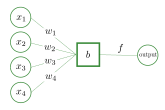
\includegraphics[width=0.5\columnwidth]{C4_cnn/neuron.pdf}
    \caption{Simple neural network}
    \label{machine:cnn:convlayer:input}
\end{subfigure}   

\begin{subfigure}[h]{\columnwidth}
    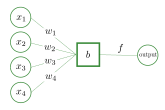
\includegraphics[width=0.5\columnwidth]{C4_cnn/neuron.pdf}
    \caption{Simple neural network}
    \label{machine:cnn:convlayer:nn}
\end{subfigure} 

\begin{subfigure}[h]{\columnwidth}
    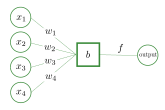
\includegraphics[width=0.5\columnwidth]{C4_cnn/neuron.pdf}
    \caption{Simple neural network}
    \label{machine:nn:convlayer:cnn}
\end{subfigure} 

\end{figure}

A convolutional layer has a number of different parameters which can be varied when setting up a model.
Below I list each of the adaptable parameters and what they do.

\begin{description}
\item[Filter size] The filter size is the size and shape of the convolutional filter. The filter does not have to be square, however must be less than the dimensions of the image.

\item[Number of filters] The number of filters can be any value. If you have $K$ filter kernels, then the convolutional layer will output $K$ filtered images.

\item[Activation function] The activation function is generally kept the same for each of the layers, however this can be set here. The different types have been explaine in Sec.~\ref{machine:nn:activation}.

\item[Stride] The stride is when the convolution is applied to every other pixel. This method reduces the size of the output by the same factor. This is not used in the rest of this work.
\end{description}

The convolutional layers with reduce the number of parameters used in each network or model, which can speed up the training procedure.
In a normal neural network the image is flattened, therefore, any information which related the location of a pixel to another is lost. 
Convolutions can keep hold of this information and look for similar patters within an image.

%%%%%%%%%
%%%%%%%%
\subsection{Max pooling layers}
%%%%%%%%%%%%
%%%%%%%%%%%

Max pooling layers are designed to reduce the size of the problem whilst holding on to as much important information as possible.
the idea of this layer is relatively simple, it reduces the image size by taking the maximum value in a reigon of a given size.
For example, in Fig.~\ref{maxpool}, the image is reduced by a 2x2 max pooling layer.

\begin{figure}
    \centering
    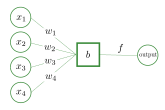
\includegraphics[width=0.5\columnwidth]{C4_cnn/neuron.pdf}
    \caption{Max pooling layer}
    \label{fig:my_label}
\end{figure}

%%%%%%%%%%%%%
%%%%%%%%%%%%%%
\subsection{CNN structure}
%%%%%%%%%%%%%%
%%%%%%%%%%%%%%

\acp{CNN} are usually structured such that they can extract larger features from an input image, then the outputs from this are passed on to be classified.
To extract the larger features any number of different convolutional layers and max-pooling layers used.
Once this then outputs $K$ images, the values are flattened into a one dimensional array an passed to a set of fully connected layers. 
This is essentially the same type of network described in Sec.~\ref{machine:nn}.
This can then classify the network into the chosen output.

\acp{CNN} are then trained in the same way as neural networks as described in Sec.~\ref{machine:nn:training}.

%%%%%%%%%%%%%%%%%%%%%%%%%%%%%%%%%%%%%%%%%%%%%%
%%%%%%%%%%%%%%%%%%%%%%%%%%%%%%%%%%%%%%%%%%%%%%%%
\section{CW search}
%%%%%%%%%%%%%%%%%%%%%%%%%%%%%%%%%%%%%%%%%%%%%%%%%
%%%%%%%%%%%%%%%%%%%%%%%%%%%%%%%%%%%%%%%%%%%%%%%




%%%%%%%%%%%%%%%
%%%%%%%%%%%%5%%
\subsection{Network structure}
%%%%%%%%%%%%%%%
%%%%%%%%%%%%%%%

\subsubsection{Viterbi statistic}

\subsubsection{Viterbi Maps}

\subsubsection{Spectrograms}

\subsubsection{Viterbi map and spectrograms}

\subsubsection{Viterbi map and Viterbi statistic}

\subsubsection{Viterbi map, Viterbi statistic and spectrograms}

%%%%%%%%%%%
%%%%%%%%%%%
\section{\label{cnn:networkvis}Network Visualisation}
%%%%%%%%%%%
%%%%%%%%%%%

Neural network are generally hard to visualise due to the large number or parameters in the network that have to be varied.
However, there are methods which can be used to see how input data is affected by the network.
This can be useful to see how the network performs when given certain types of data and gives some insight into how the networks work

In the examples above we use \acp{CNN}, the first few layers of this are build using convolutional filters.
The filters weights should ideally correspond to the shape of the feature which one wants to extract from the image. 
Generally this is only useful to picture at the first layer as the network can make subsequent layer and representations quite abstract.



\begin{figure}
	\centering
	\includegraphics[width=\textwidth]{testimg.png}
	\caption{different types of instrumental line which appear in SOAP spectrograms}
	\label{detchar:line:psd}
\end{figure}


%%%%%%%%%
%%%%%%%%%%%
\section{Data and simulations}
%%%%%%%%%%
%%%%%%%%%%%